
\begin{frame}{AdaBoost: Weak learner}
\begin{itemize}
    \item \textbf{Decision ``stumps''}:
    \begin{itemize}
        \item 1-level decision tree
        \item A decision boundary based on one feature
        \begin{itemize}
            \item E.g.: If someone is not a smoker, then predict them to live past 80 years old
        \end{itemize}
        \item Building blocks of AdaBoost algorithm
        \item \textbf{Decision stump} is a \textbf{weak learner}
    \end{itemize}
\end{itemize}

\begin{figure}[h]
    \centering
    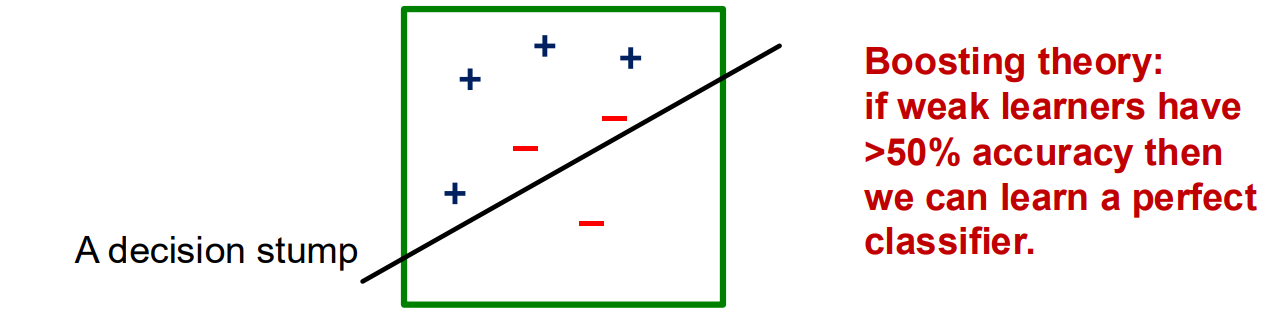
\includegraphics[width=0.85\textwidth]{images/decision-trees/decision-trees-16.png}
\end{figure}

\end{frame}


\begin{frame}{Build Decision Trees with AdaBoost}
Suppose we have training data 
\[
\left\{ (x_i, y_i) \right\}_{i=1}^N, \quad y_i \in \{1, -1\}
\]

\begin{itemize}
    \item Initialize equal weights for all observations: \quad \( w_i = \frac{1}{N} \)

    \item At each iteration \( t \):
    \begin{enumerate}
        \item Train a stump \( G_t \) using data weighted by \( w_i \)
        \item Compute the \textbf{misclassification error} adjusted by \( w_i \)
        \item Compute the weight of the current tree \( \alpha_t \)
        \item Reweight each observation based on prediction accuracy
    \end{enumerate}
\end{itemize}
\end{frame}


\begin{frame}{Update Step}
\begin{itemize}
    \item Calculate the weighted misclassification error:
    \[
    \text{err}_t = \frac{\sum_{i=1}^{N} w_i \, I(y_i \neq G_t(x_i))}{\sum_{i=1}^{N} w_i}
    \]

    \item Use the error score to weight the current tree in the final classifier:
    \[
    \alpha_t = \log\left(\frac{1 - \text{err}_t}{\text{err}_t}\right)
    \]
    A classifier with 50\% accuracy is given a weight of zero;

    \item Use misclassification error and tree weight to reweight the training data:
    \[
    w_i \leftarrow w_i \exp\left[\alpha_t \, I(y_i \neq G_t(x_i))\right]
    \]
    Training instances that are harder to classify get higher weight
\end{itemize}
\end{frame}


\begin{frame}{Final Prediction}
\begin{itemize}
    \item Final prediction is a weighted sum of the predictions from each stump:
    \[
    G(x) = \text{sign} \left[ \sum_{t=1}^{T} \alpha_t G_t(x) \right]
    \]
    
    \item More accurate trees are weighted higher in the final model
\end{itemize}
\end{frame}


\begin{frame}{AdaBoost: Summary}
\begin{enumerate}
    \item Initialize the observation weights \( w_i = \frac{1}{N},\; i = 1, 2, \ldots, N \).
    
    \item For \( m = 1 \) to \( M \):
    \begin{enumerate}
        \item Fit a classifier \( G_m(x) \) to the training data using weights \( w_i \).
        
        \item Compute
        \[
        \text{err}_m = \frac{\sum_{i=1}^{N} w_i \mathbb{I}(y_i \ne G_m(x_i))}{\sum_{i=1}^{N} w_i}
        \]
        
        \item Compute \( \alpha_m = \log \left( \frac{1 - \text{err}_m}{\text{err}_m} \right) \).
        
        \item Set \( w_i \leftarrow w_i \cdot \exp \left[ \alpha_m \cdot \mathbb{I}(y_i \ne G_m(x_i)) \right],\quad i = 1, 2, \ldots, N \).
    \end{enumerate}

    \item Output 
    \[
    G(x) = \text{sign} \left[ \sum_{m=1}^{M} \alpha_m G_m(x) \right]
    \]
\end{enumerate}
\end{frame}

\begin{frame}{AdaBoost Conclusion}
\begin{itemize}
    \item \textbf{Iteratively train weak learners (decision stumps) to form a strong model:}
    \begin{itemize}
        \item Trees with high accuracy are given more weights in the final model
        \item Misclassified data get higher weights in the next iteration
    \end{itemize}

    \item AdaBoost is the equivalent to additive training with the exponential loss (Friedman et al. 2000)

    \item We will talk about additive training in more general scenarios next!
\end{itemize}
\end{frame}